% -*-coding: iso-latin-1  -*-
%---------------------------------------------------------------------
%
%                          Ap�ndice 5
%
%---------------------------------------------------------------------

\chapter{Diagrama de clases inicial del Proyecto}
	\label{ap1:classDiagra_v0}
			El presente documento puede ser consultado en el repositorio GitHub del proyecto\footnote{Acceso al material online: https://github.com/ERicBastida/BEcopter-Informe-Final/blob/master/Imagenes/ClassDiagram.png}.
	 
			\begin{figure}[!h]
				\centering
				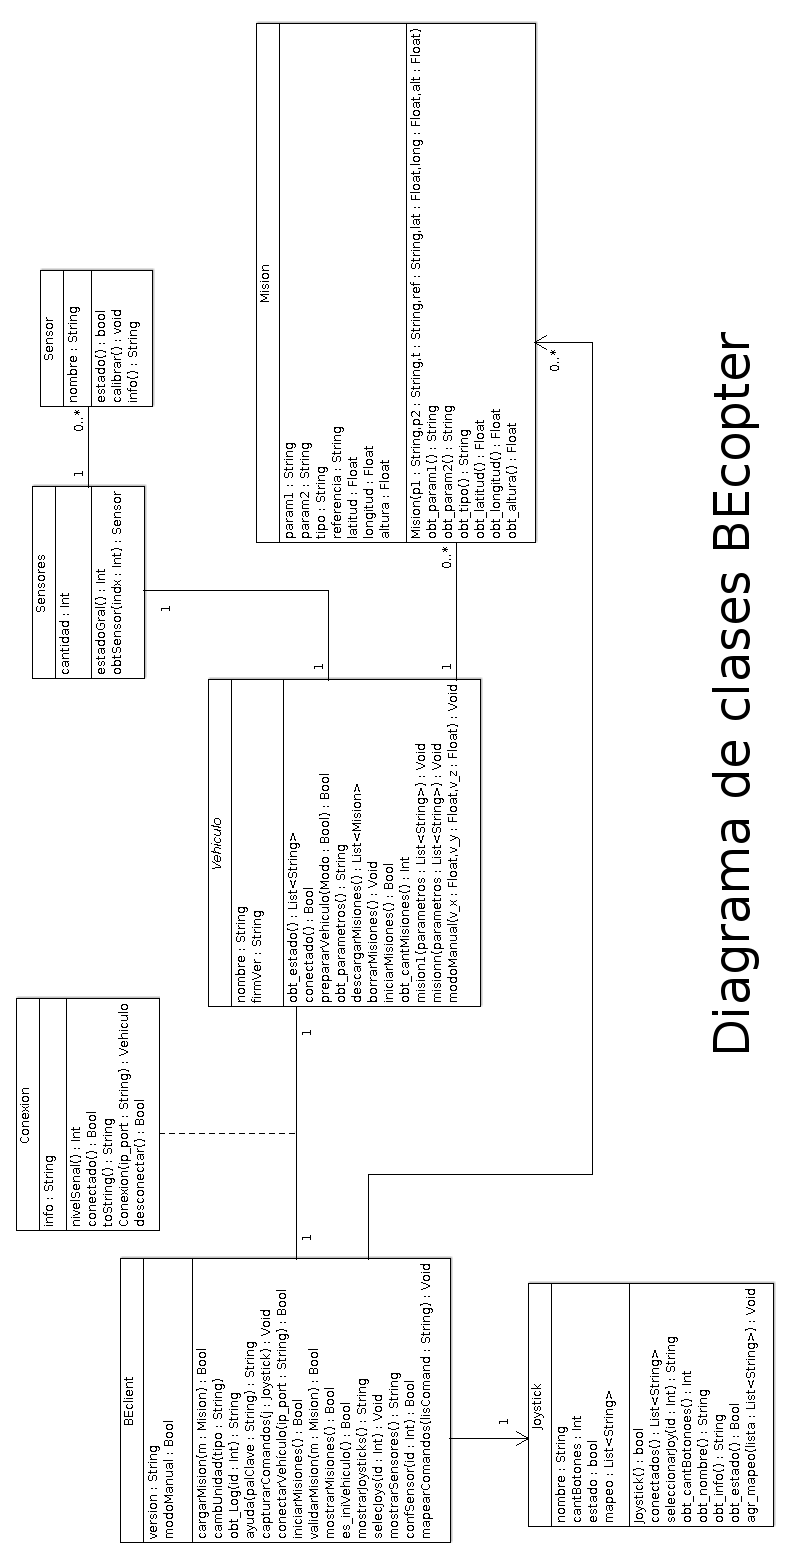
\includegraphics[width=\linewidth, height=0.93\textheight]{Apendices/Apendice_files/DC_v0}
				\caption{Diagrama de clases inicial de BEcopter. }	
			\end{figure}


% Variable local para emacs, para  que encuentre el fichero maestro de
% compilaci�n y funcionen mejor algunas teclas r�pidas de AucTeX
%%%
%%% Local Variables:
%%% mode: latex
%%% TeX-master: "../Tesis.tex"
%%% End:
